\documentclass{article}
\usepackage{graphicx} % Required for inserting images
\usepackage{hyperref}
\usepackage{adjustbox} % Allows for adjustment of box sizes
\usepackage[table,xcdraw]{xcolor}
\usepackage{colortbl}
\usepackage{booktabs, 
            multirow, threeparttable}   % new
\usepackage{siunitx}                    % new
\usepackage{xparse}                     % new
\usepackage{lipsum}
\usepackage{fancyhdr}
\usepackage{subcaption}

\NewExpandableDocumentCommand\mcc{O{1}m}
    {\multicolumn{#1}{c}{#2}}

\usepackage{lipsum}                     % for dummy text

\title{Data Key and Extended Table}
\author{Alex Wellman}
\begin{document}

\pagestyle{fancy}
\fancyhf{}
\fancyhf[EHC]{Variable Key and Extended Table}
% \fancyhf[EFC]{Variable Key and Extended Table}
% \fancyhf[OFC]{Variable Key and Extended Table}
\fancyhf[OHC]{Variable Key and Extended Table}

\begin{table}[H!]
\caption{Variable Key}
\centering
\begin{adjustbox}{width=\textwidth,center}
\begin{tabular}{lll}
\hline
Variable & Definition & Data  \\
\hline
Y\textsuperscript{‡} & GDP & \href{https://fred.stlouisfed.org/series/GDPC1}{link} \\
C\textsuperscript{*}\textsuperscript{†} & Consumption & \href{https://fred.stlouisfed.org/series/PCEC96}{link} \\
G\textsuperscript{‡} & Government Expenditure & \href{https://fred.stlouisfed.org/series/GCEC1}{link} \\
I\textsuperscript{‡} & Investment & \href{https://fred.stlouisfed.org/series/GPDIC1}{link} \\
N\textsuperscript{*} & Labor Force & \href{https://fred.stlouisfed.org/series/PAYEMS}{link}  \\
D\textsuperscript{†} & Household Debt & \href{https://fred.stlouisfed.org/series/HCCSDODNS}{link}\\
BG\textsuperscript{†} & Government Debt &  \href{https://fred.stlouisfed.org/series/GFDEBTN}{link} \\
w_{manf.}\textsuperscript{*†}  & Ave. Manf. Wage (Real) & \href{https://fred.stlouisfed.org/series/CES3000000008}{link} \\
W_{manf.}\textsuperscript{*}  & Ave. Manf. Wage (Nominal) & \href{https://fred.stlouisfed.org/series/CES3000000008}{link} \\
tax\textsuperscript{†} & Income Tax & \href{https://fred.stlouisfed.org/series/A074RC1Q027SBEA}{link} \\
BK & Number of Bankruptcies & xlsx, annual, total (interpolated to quarterly)\\ 
CO_{level} & Consumer Loans Charged-Off & xlsx, summary, column H\\ 
CPI_{level}\textsuperscript{*} & CPI Urban (Index 1984=100) & \href{https://fred.stlouisfed.org/series/CPIAUCSL}{link}   \\ 
PCE_{level}\textsuperscript{*} & PCEPI (Index 2017=100) & \href{https://fred.stlouisfed.org/series/PCEPI}{link}    \\ 

\hline

CO_{rate} & Charge-Off Rate on Consumer Loans & \href{https://fred.stlouisfed.org/series/CORCACBS}{link}  \\ 
CPI_{rate} & CPI Inflation & \% change of $CPI_{level}$ from prev. year   \\ 
PCE_{rate} & PCE Inflation & \% change of $PCE_{level}$ from prev. year   \\ 
i\textsuperscript{*} & Interest Rate & \href{https://fred.stlouisfed.org/series/FEDFUNDS}{link}\\
\pi^{W}_{manf.}\textsuperscript{*} & Manf. Wage Inflation &  \% change of nominal $W_{manf.}$ from prev. year \\
BK/N &  Bankruptcy / Labor Force & xlsx, annual, total and \href{https://fred.stlouisfed.org/series/PAYEMS}{link} \\
BG/Y &  Gov. Debt / Output & \href{https://fred.stlouisfed.org/series/GFDEBTN}{link} and \href{https://fred.stlouisfed.org/series/GDPC1}{link} \\
D/Y &  Household Debt / Output & \href{https://fred.stlouisfed.org/series/HCCSDODNS}{link} and \href{https://fred.stlouisfed.org/series/GDP}{link} \\
\hline \\
\multicolumn{3}{l}{\footnotesize{Data is 1985Q1 to 2017Q4}}\\
\multicolumn{3}{l}{\footnotesize{Raw data is quarterly unless specified and all final data is quarterly}}\\
\multicolumn{3}{l}{\textsuperscript{*}\footnotesize{Monthly data averaged to quarterly}}\\
\multicolumn{3}{l}{\textsuperscript{†}\footnotesize{Deflated using CPI}}\\
\multicolumn{3}{l}{\textsuperscript{‡}\footnotesize{Deflated using FRED provided deflator}}\\
\end{tabular}
\end{adjustbox}
\end{table}

\begin{table}[H!]
\caption{SD and Correlations}
\begin{adjustbox}{width=\textwidth,center}
\begin{tabular}{l|rrr|rrr|rrr}
\toprule
 \multicolumn{}{r}{}  & \multicolumn{3}{l}{Non-Filtered and HP Filtered} & \multicolumn{3}{l}{Annual Change} & \multicolumn{3}{l}{Annualized Quarterly Change} \\
Variable & SD \% & Cor(y, x) & Cor(x, x_{t-4}) & SD \% & Cor(y, x) & Cor(x, x_{t-4}) & SD \% & Cor(y, x) & Cor(x, x_{t-4}) \\ \hline
\midrule
& \multicolumn{3}{c|}{Filtered, Levels} & & & & & & \\
Y & 1.040 & 1.000 & 0.317 & 1.626 & 1.000 & 0.302 & 2.310 & 1.000 & 0.124 \\
C & 0.682 & 0.878 & -0.017 & 1.448 & 0.905 & 0.378 & 1.798 & 0.736 & 0.133 \\
G & 1.224 & -0.420 & 0.467 & 1.995 & -0.038 & 0.568 & 3.124 & 0.190 & 0.350 \\
I & 5.425 & 0.894 & 0.304 & 7.895 & 0.836 & 0.157 & 11.934 & 0.744 & -0.033 \\
N & 1.104 & 0.808 & 0.522 & 1.602 & 0.787 & 0.573 & 1.725 & 0.610 & 0.466 \\
D & 2.502 & 0.241 & 0.485 & 3.780 & 0.381 & 0.565 & 4.871 & 0.222 & 0.343 \\
BG & 2.372 & -0.394 & 0.372 & 4.113 & -0.484 & 0.525 & 5.940 & -0.358 & 0.430 \\
w_{manf.} & 0.789 & -0.449 & 0.199 & 1.247 & -0.240 & 0.160 & 2.087 & -0.184 & -0.107 \\
W_{manf.} & 0.458 & -0.515 & 0.361 & 0.773 & -0.047 & 0.490 & 1.142 & 0.010 & 0.128 \\
tax & 7.020 & 0.719 & 0.350 & 9.520 & 0.587 & 0.183 & 18.405 & 0.247 & 0.060 \\
BK & 14.256 & -0.496 & 0.213 & 20.818 & -0.185 & 0.053 & 26.792 & -0.154 & -0.131 \\
CO_{level} & 18.125 & -0.559 & 0.459 & 22.819 & -0.315 & 0.343 & 50.281 & -0.134 & 0.472 \\
CPI_{level} & 0.711 & 0.166 & 0.123 & 1.283 & 0.205 & 0.338 & 1.996 & 0.199 & 0.050 \\
PCE_{level} & 0.561 & 0.277 & 0.149 & 1.088 & 0.227 & 0.437 & 1.549 & 0.236 & 0.113 \\
\hline
& \multicolumn{3}{c|}{Non-Filtered, Rates} & & & & & & \\
CO_{rate} & 1.051 & -0.400 & 0.755 & 0.737 & -0.400 & 0.302 & 1.127 & -0.270 & 0.070 \\
CPI_{rate} & 1.315 & 0.399 & 0.341 & 1.526 & 0.406 & -0.429 & 2.847 & 0.270 & -0.527 \\
PCE_{rate} & 1.111 & 0.394 & 0.441 & 1.190 & 0.446 & -0.406 & 2.127 & 0.297 & -0.518 \\
i & 2.842 & 0.370 & 0.875 & 1.404 & 0.529 & 0.265 & 1.748 & 0.382 & 0.123 \\
\pi^{W}_{manf.} & 0.812 & -0.032 & 0.441 & 0.852 & -0.021 & -0.289 & 1.562 & -0.023 & -0.396 \\
\cline{2-4}
& \multicolumn{3}{c|}{Filtered, Rates} & & & & & & \\
BK/N & 14.838 & -0.536 & 0.245 & 0.188 & -0.257 & 0.042 & 0.234 & -0.179 & -0.180 \\
BG/Y & 2.829 & -0.697 & 0.429 & 3.412 & -0.726 & 0.569 & 4.679 & -0.620 & 0.445 \\
D/Y & 2.414 & -0.180 & 0.415 & 0.507 & -0.047 & 0.381 & 0.705 & -0.229 & 0.161 \\
\bottomrule

\multicolumn{10}{l}{\footnotesize{Filtered data: HP filter cycle component, 1600}}\\
\multicolumn{10}{l}{\footnotesize{$Cor(x, x_{t-4})$ indicates the correlation between x at t and the previous year}}\\
\multicolumn{10}{l}{\footnotesize{Annual Change: \% change from previous year; x $= 100*(log(x)_t-log(x)_{t-4})$ above middle line and x $= x_t-x_{t-4}$ below middle line  }}\\
\multicolumn{10}{l}{\footnotesize{Annualized Quarterly Change: \% change from previous quarter annualized; x $= 400*(log(x)_t-log(x)_{t-1})$ above middle line}}\\
\multicolumn{10}{l}{\footnotesize{and x $= 4*(x_t-x_{t-1})$ below middle line  }}\\

\end{tabular}
\end{adjustbox}
\end{table}

\begin{figure}[H!]
\centering
% First row of two images
\begin{subfigure}{0.45\textwidth}
  \centering
  \includegraphics[width=\linewidth]{D_cycle_vs_Y_cycle.png}
\end{subfigure}%
\hspace{0.05\textwidth} % Space between the images
\begin{subfigure}{0.45\textwidth}
  \centering
  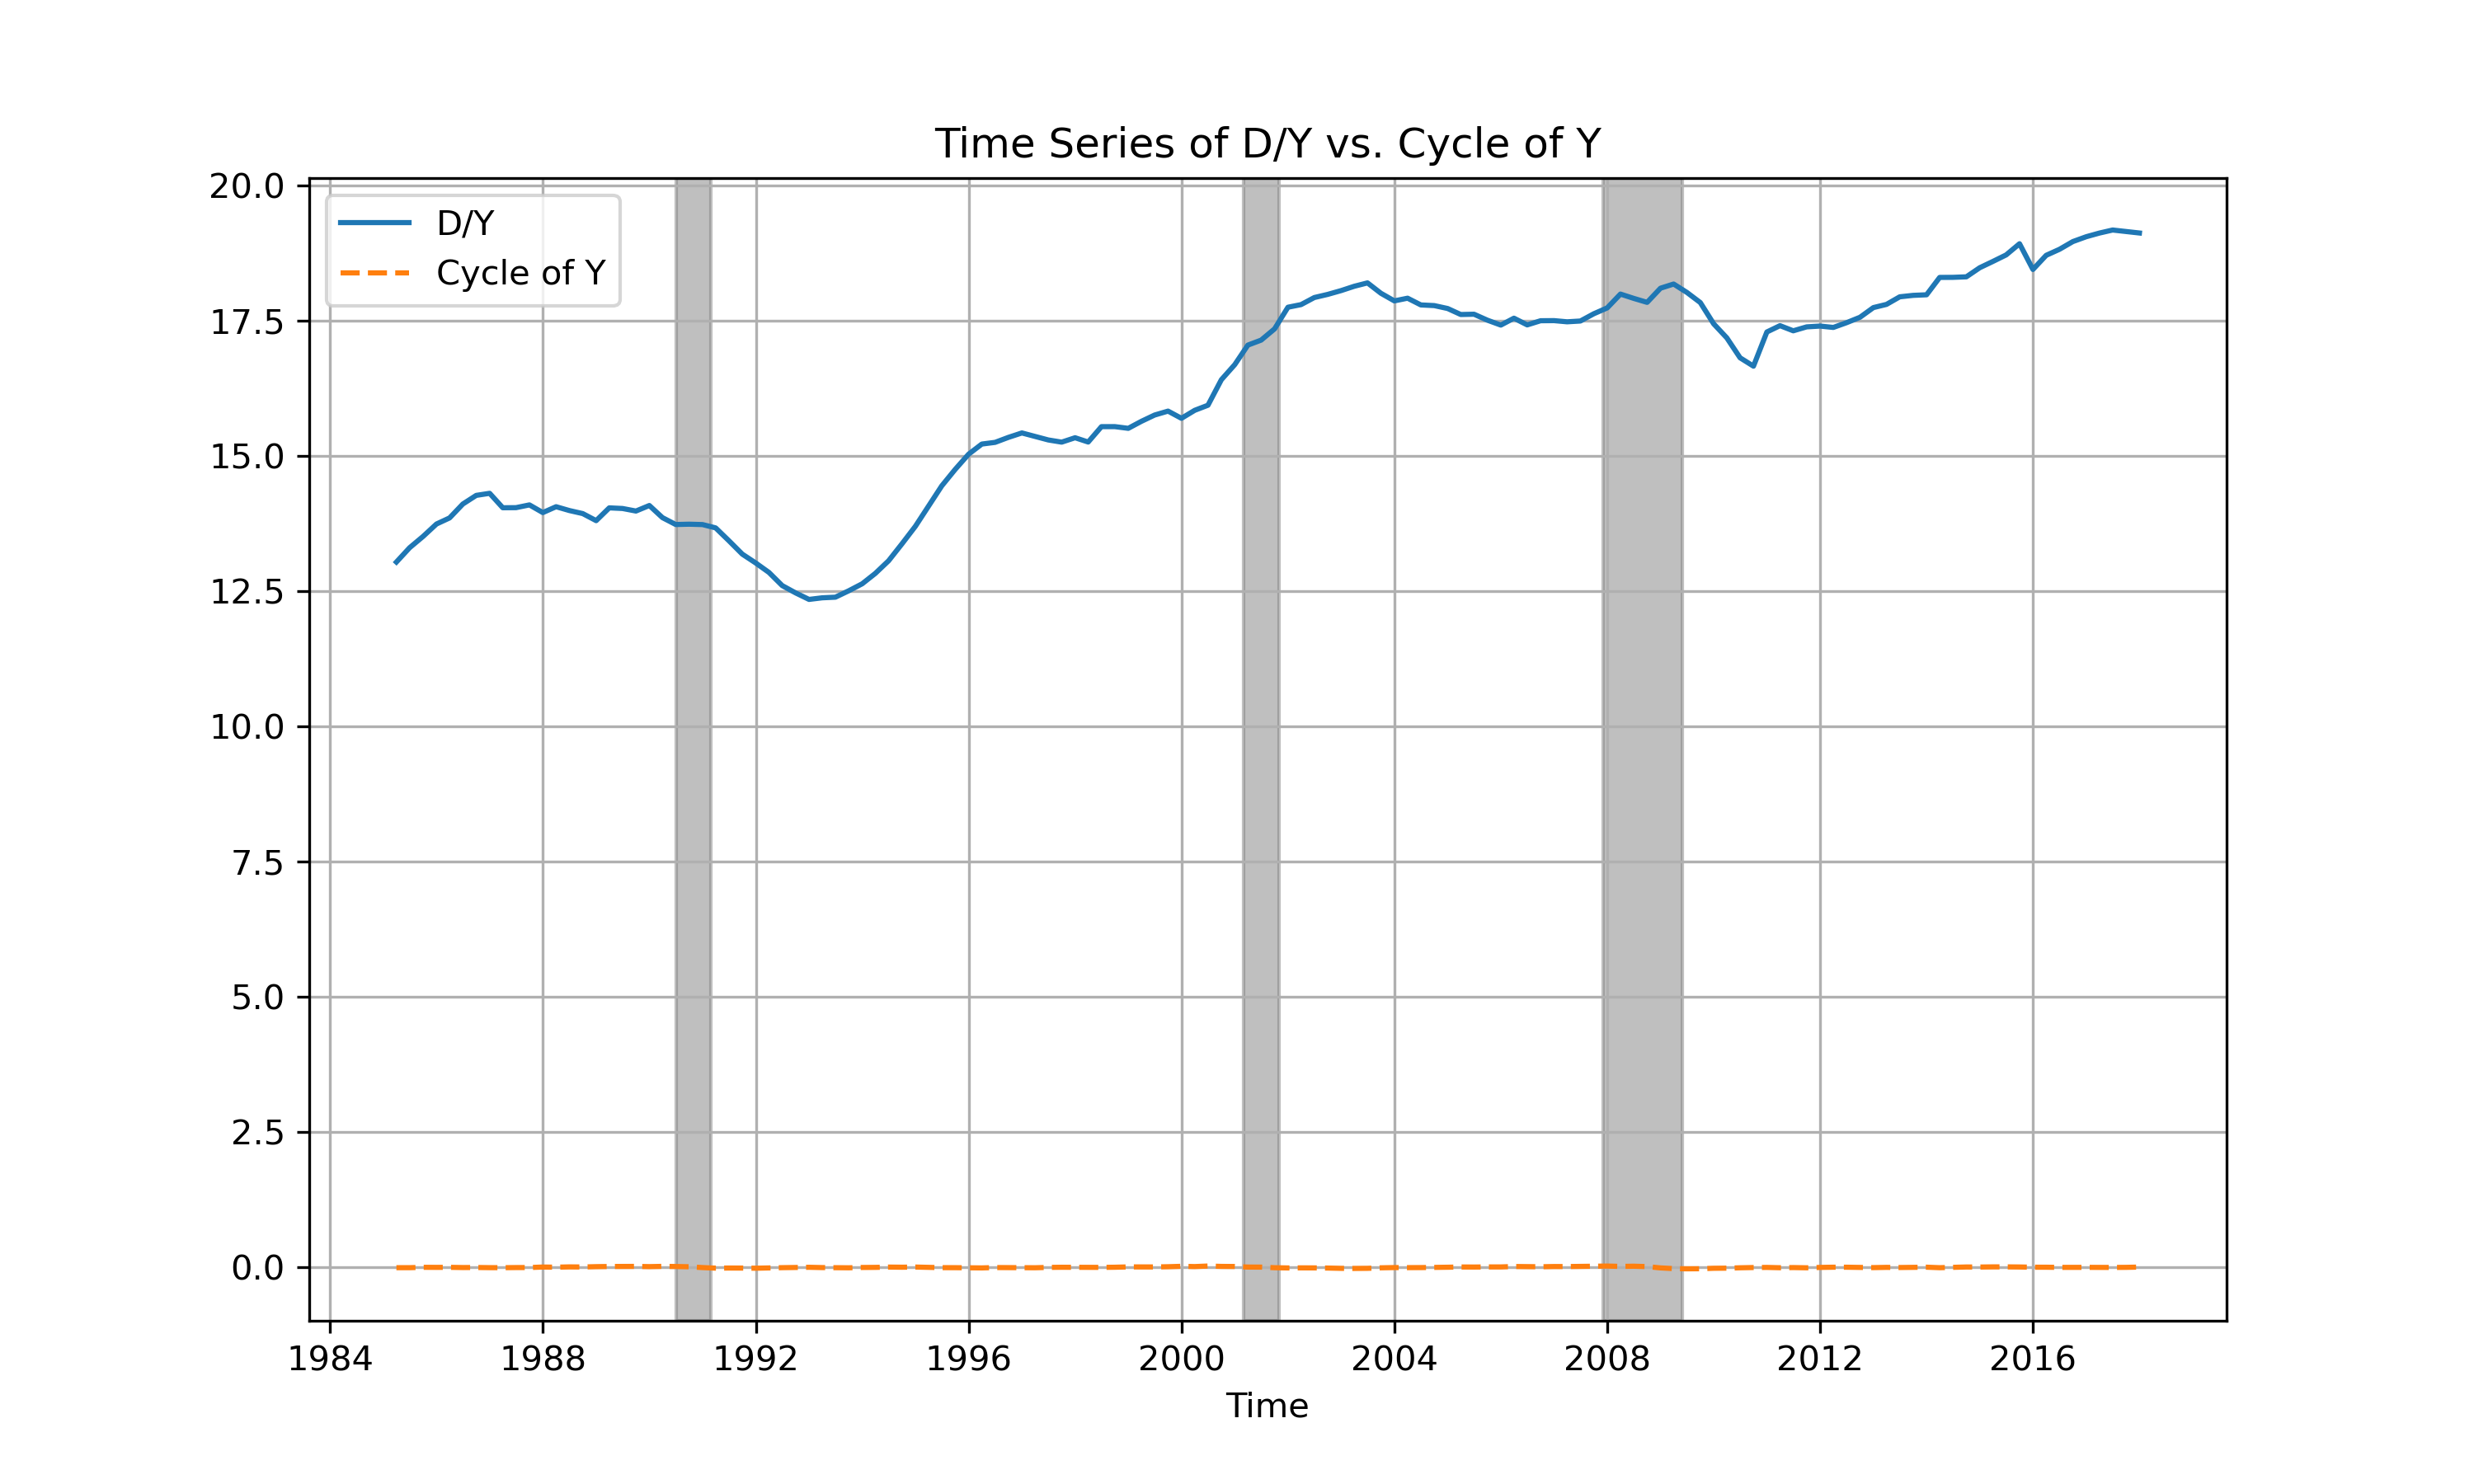
\includegraphics[width=\linewidth]{D_Y_vs_Y_cycle.png}
\end{subfigure}

\vspace{1em} % Space between the rows

% Second row of two images
\begin{subfigure}{0.45\textwidth}
  \centering
  \includegraphics[width=\linewidth]{CPI_cycle_vs_Y_cycle.png}
\end{subfigure}%
\hspace{0.05\textwidth} % Space between the images
\begin{subfigure}{0.45\textwidth}
  \centering
  \includegraphics[width=\linewidth]{CPI Rate_vs_Y_cycle.png}
\end{subfigure}

\vspace{1em} % Space between the rows

% Third row of two images
\begin{subfigure}{0.45\textwidth}
  \centering
  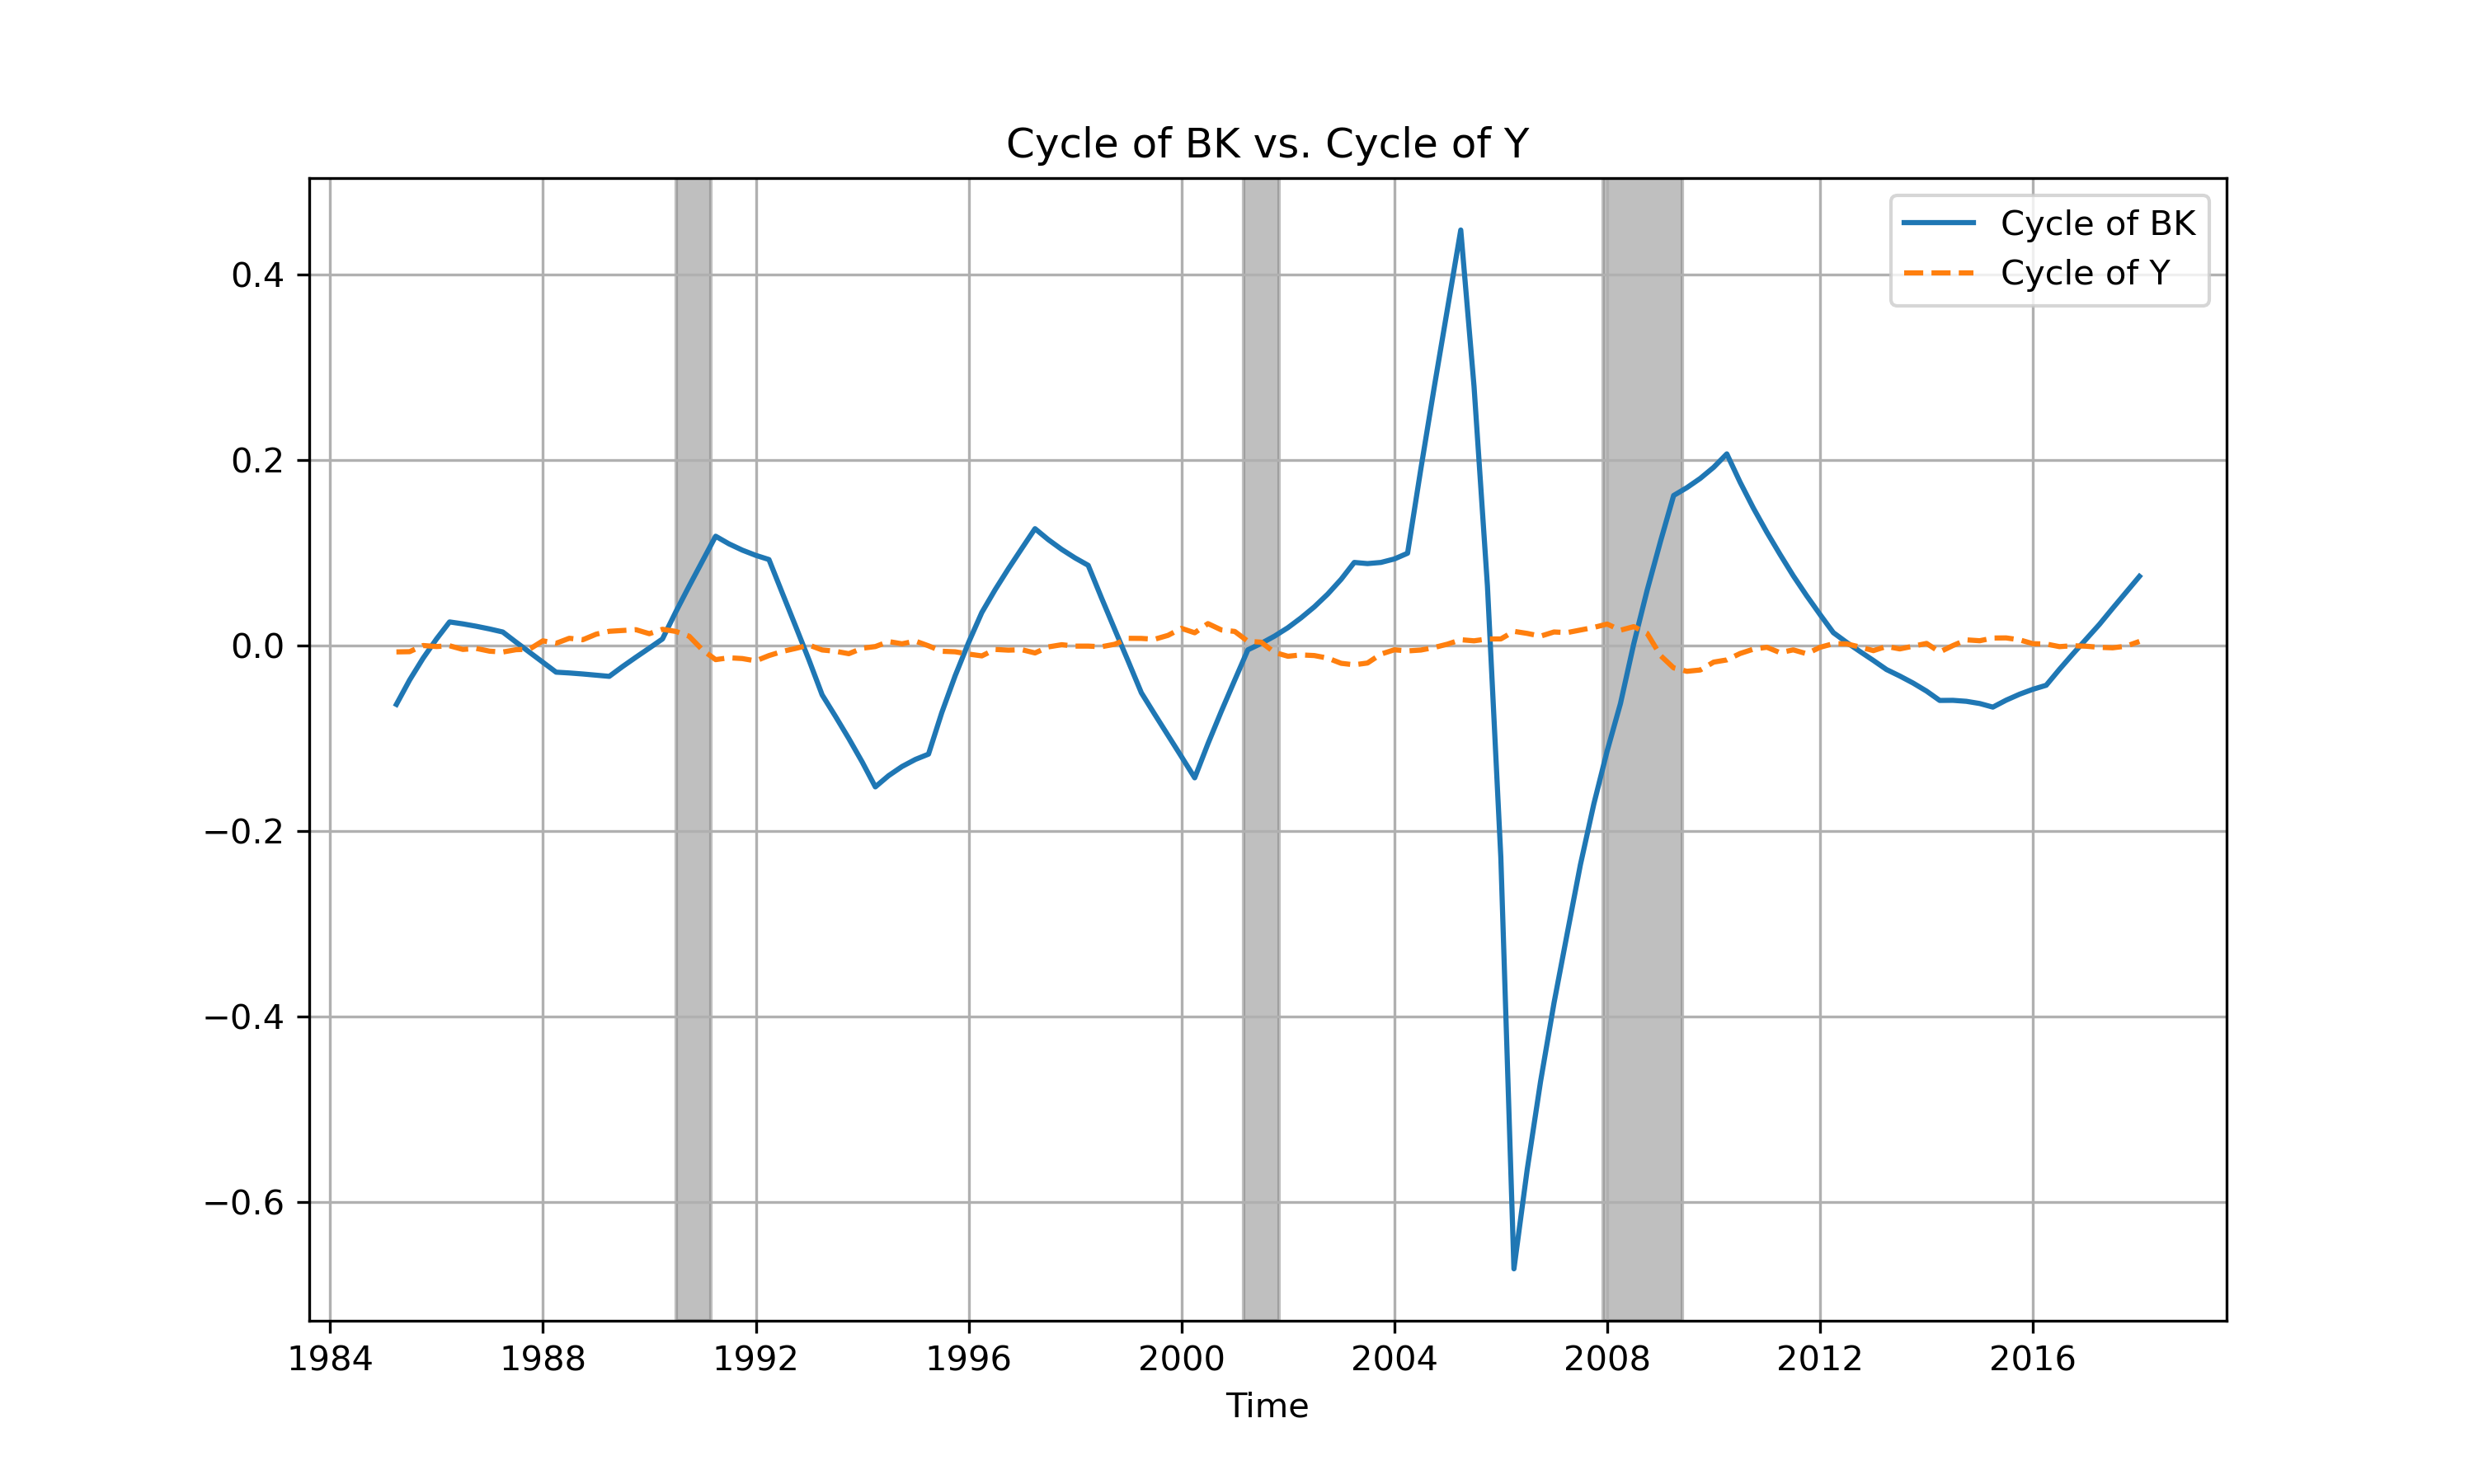
\includegraphics[width=\linewidth]{BK_cycle_vs_Y_cycle.png}
\end{subfigure}%
\hspace{0.05\textwidth} % Space between the images
\begin{subfigure}{0.45\textwidth}
  \centering
  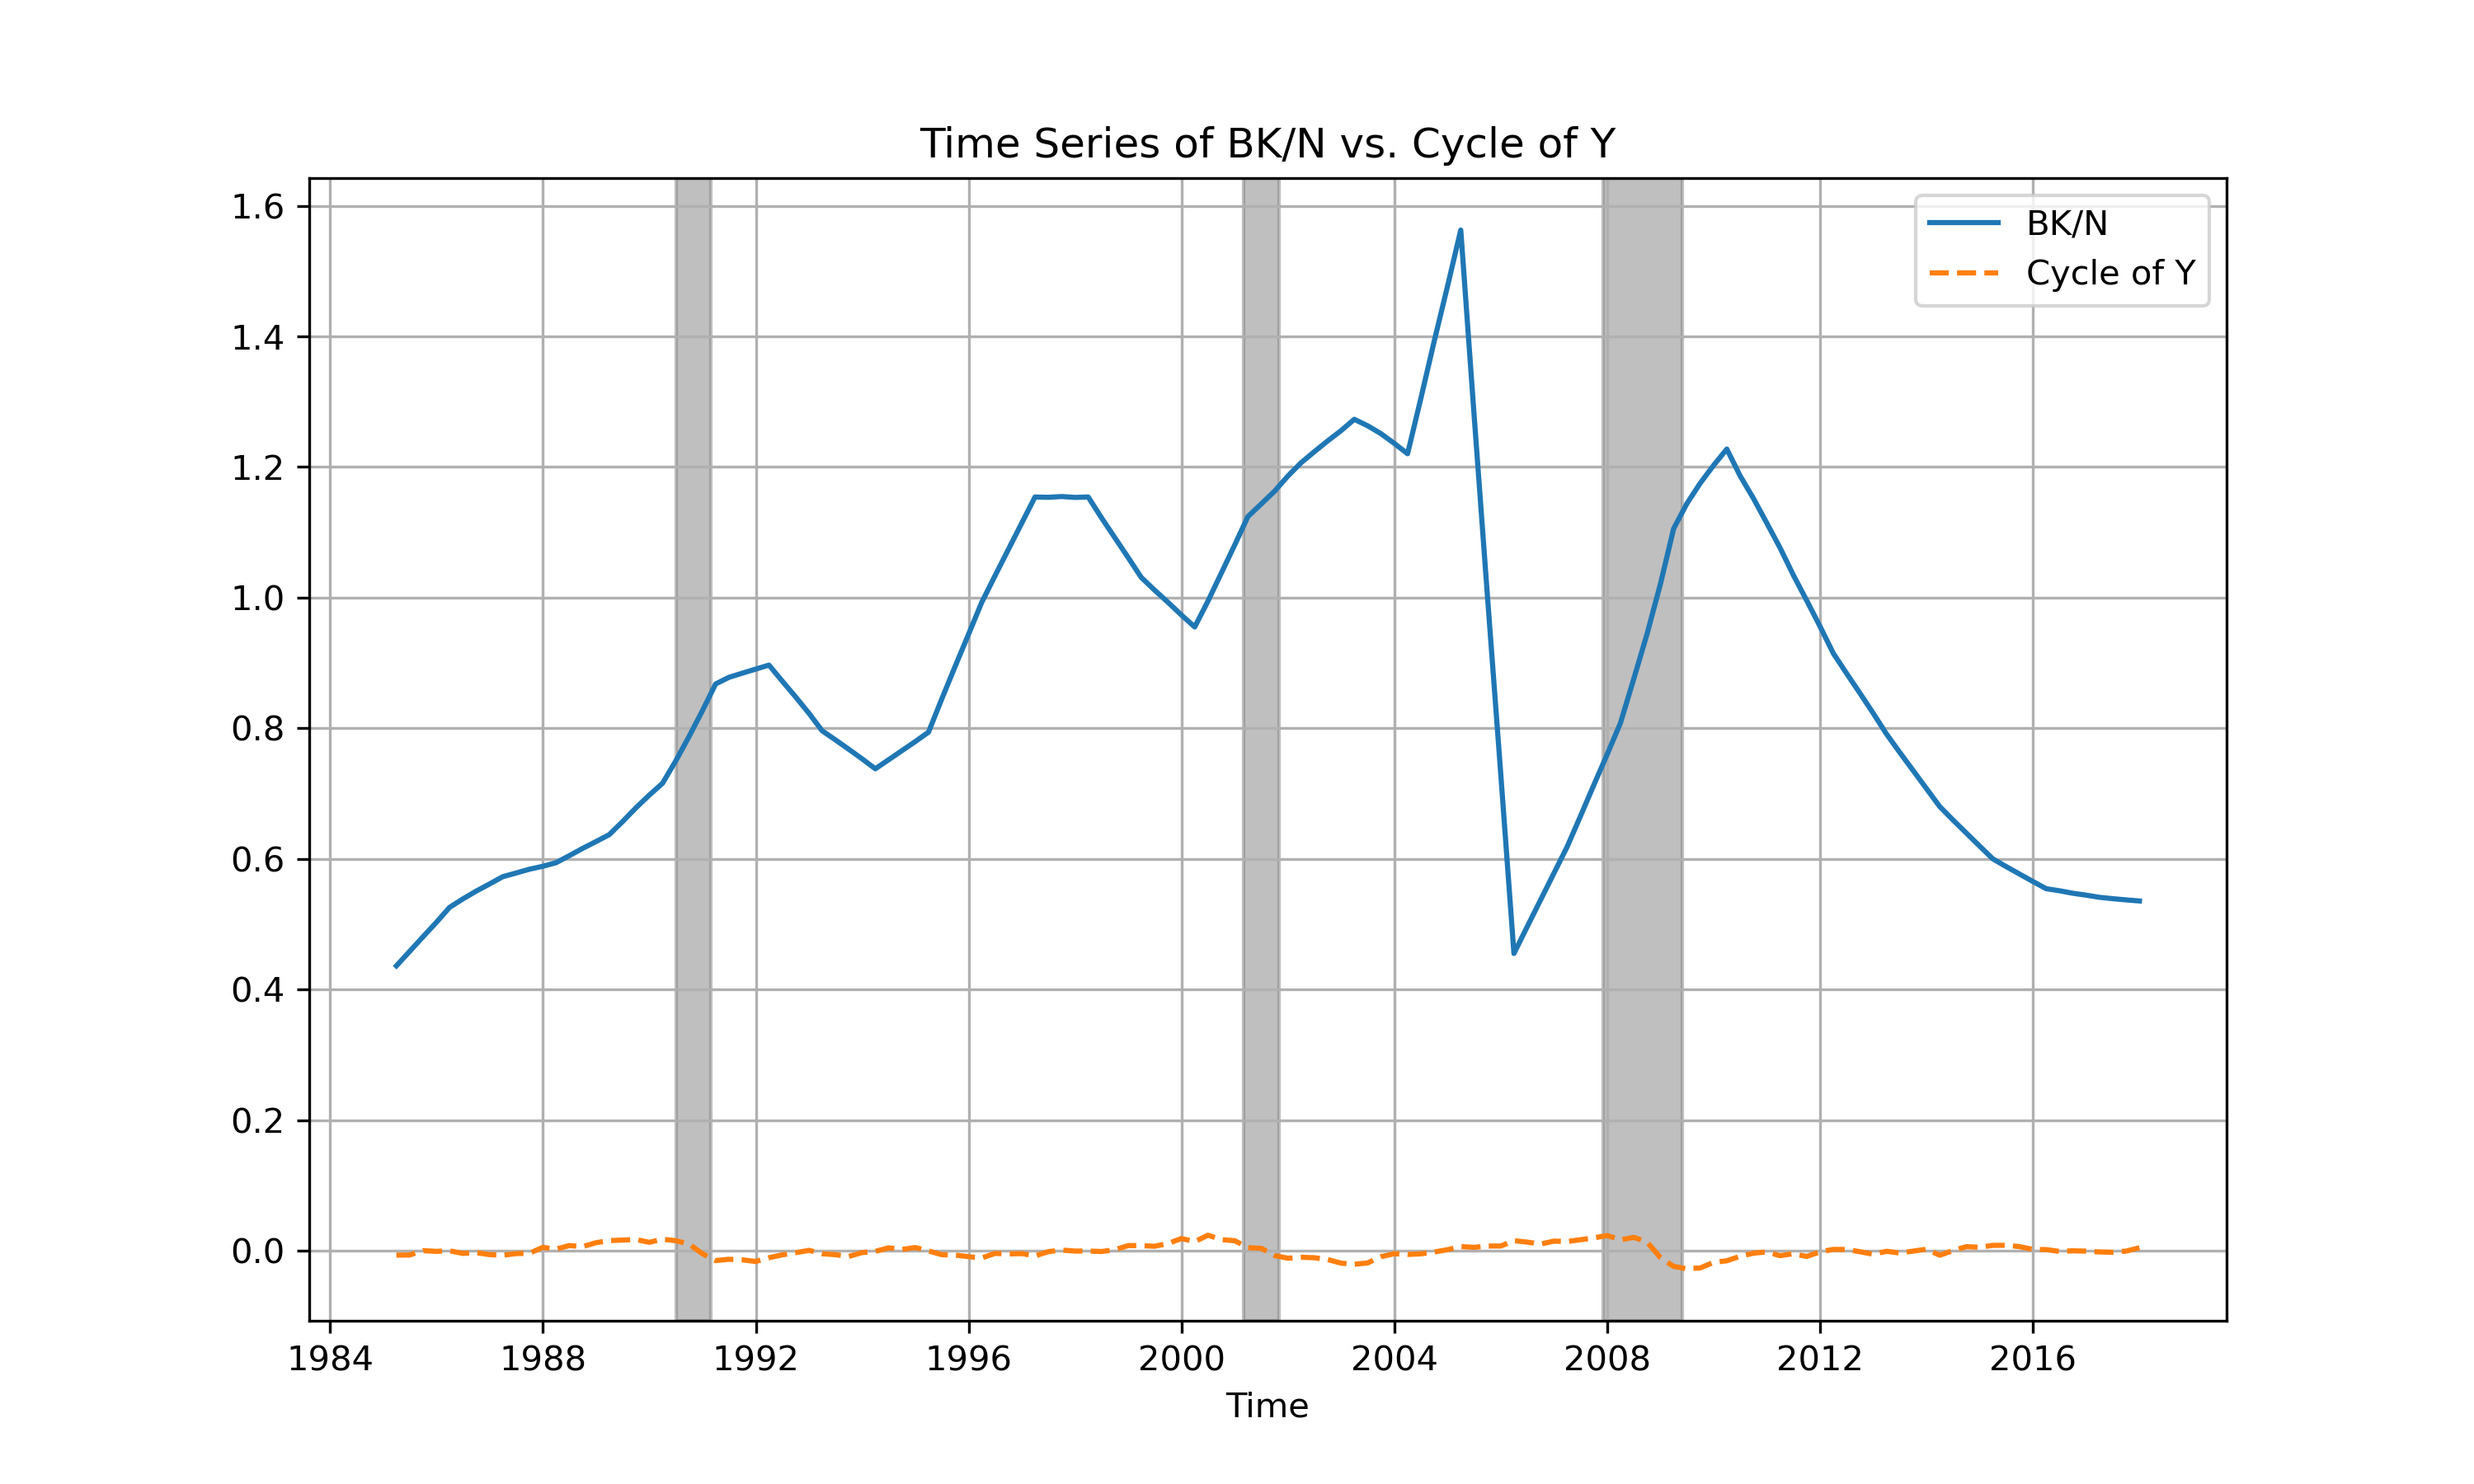
\includegraphics[width=\linewidth]{BK_N_vs_Y_cycle.png}
\end{subfigure}
\end{figure}


\begin{figure}[H!]
\centering
% First row of two images
\begin{subfigure}{0.45\textwidth}
  \centering
  \includegraphics[width=\linewidth]{D_annual_change_vs_Y.png}
\end{subfigure}%
\hspace{0.05\textwidth} % Space between the images
\begin{subfigure}{0.45\textwidth}
  \centering
  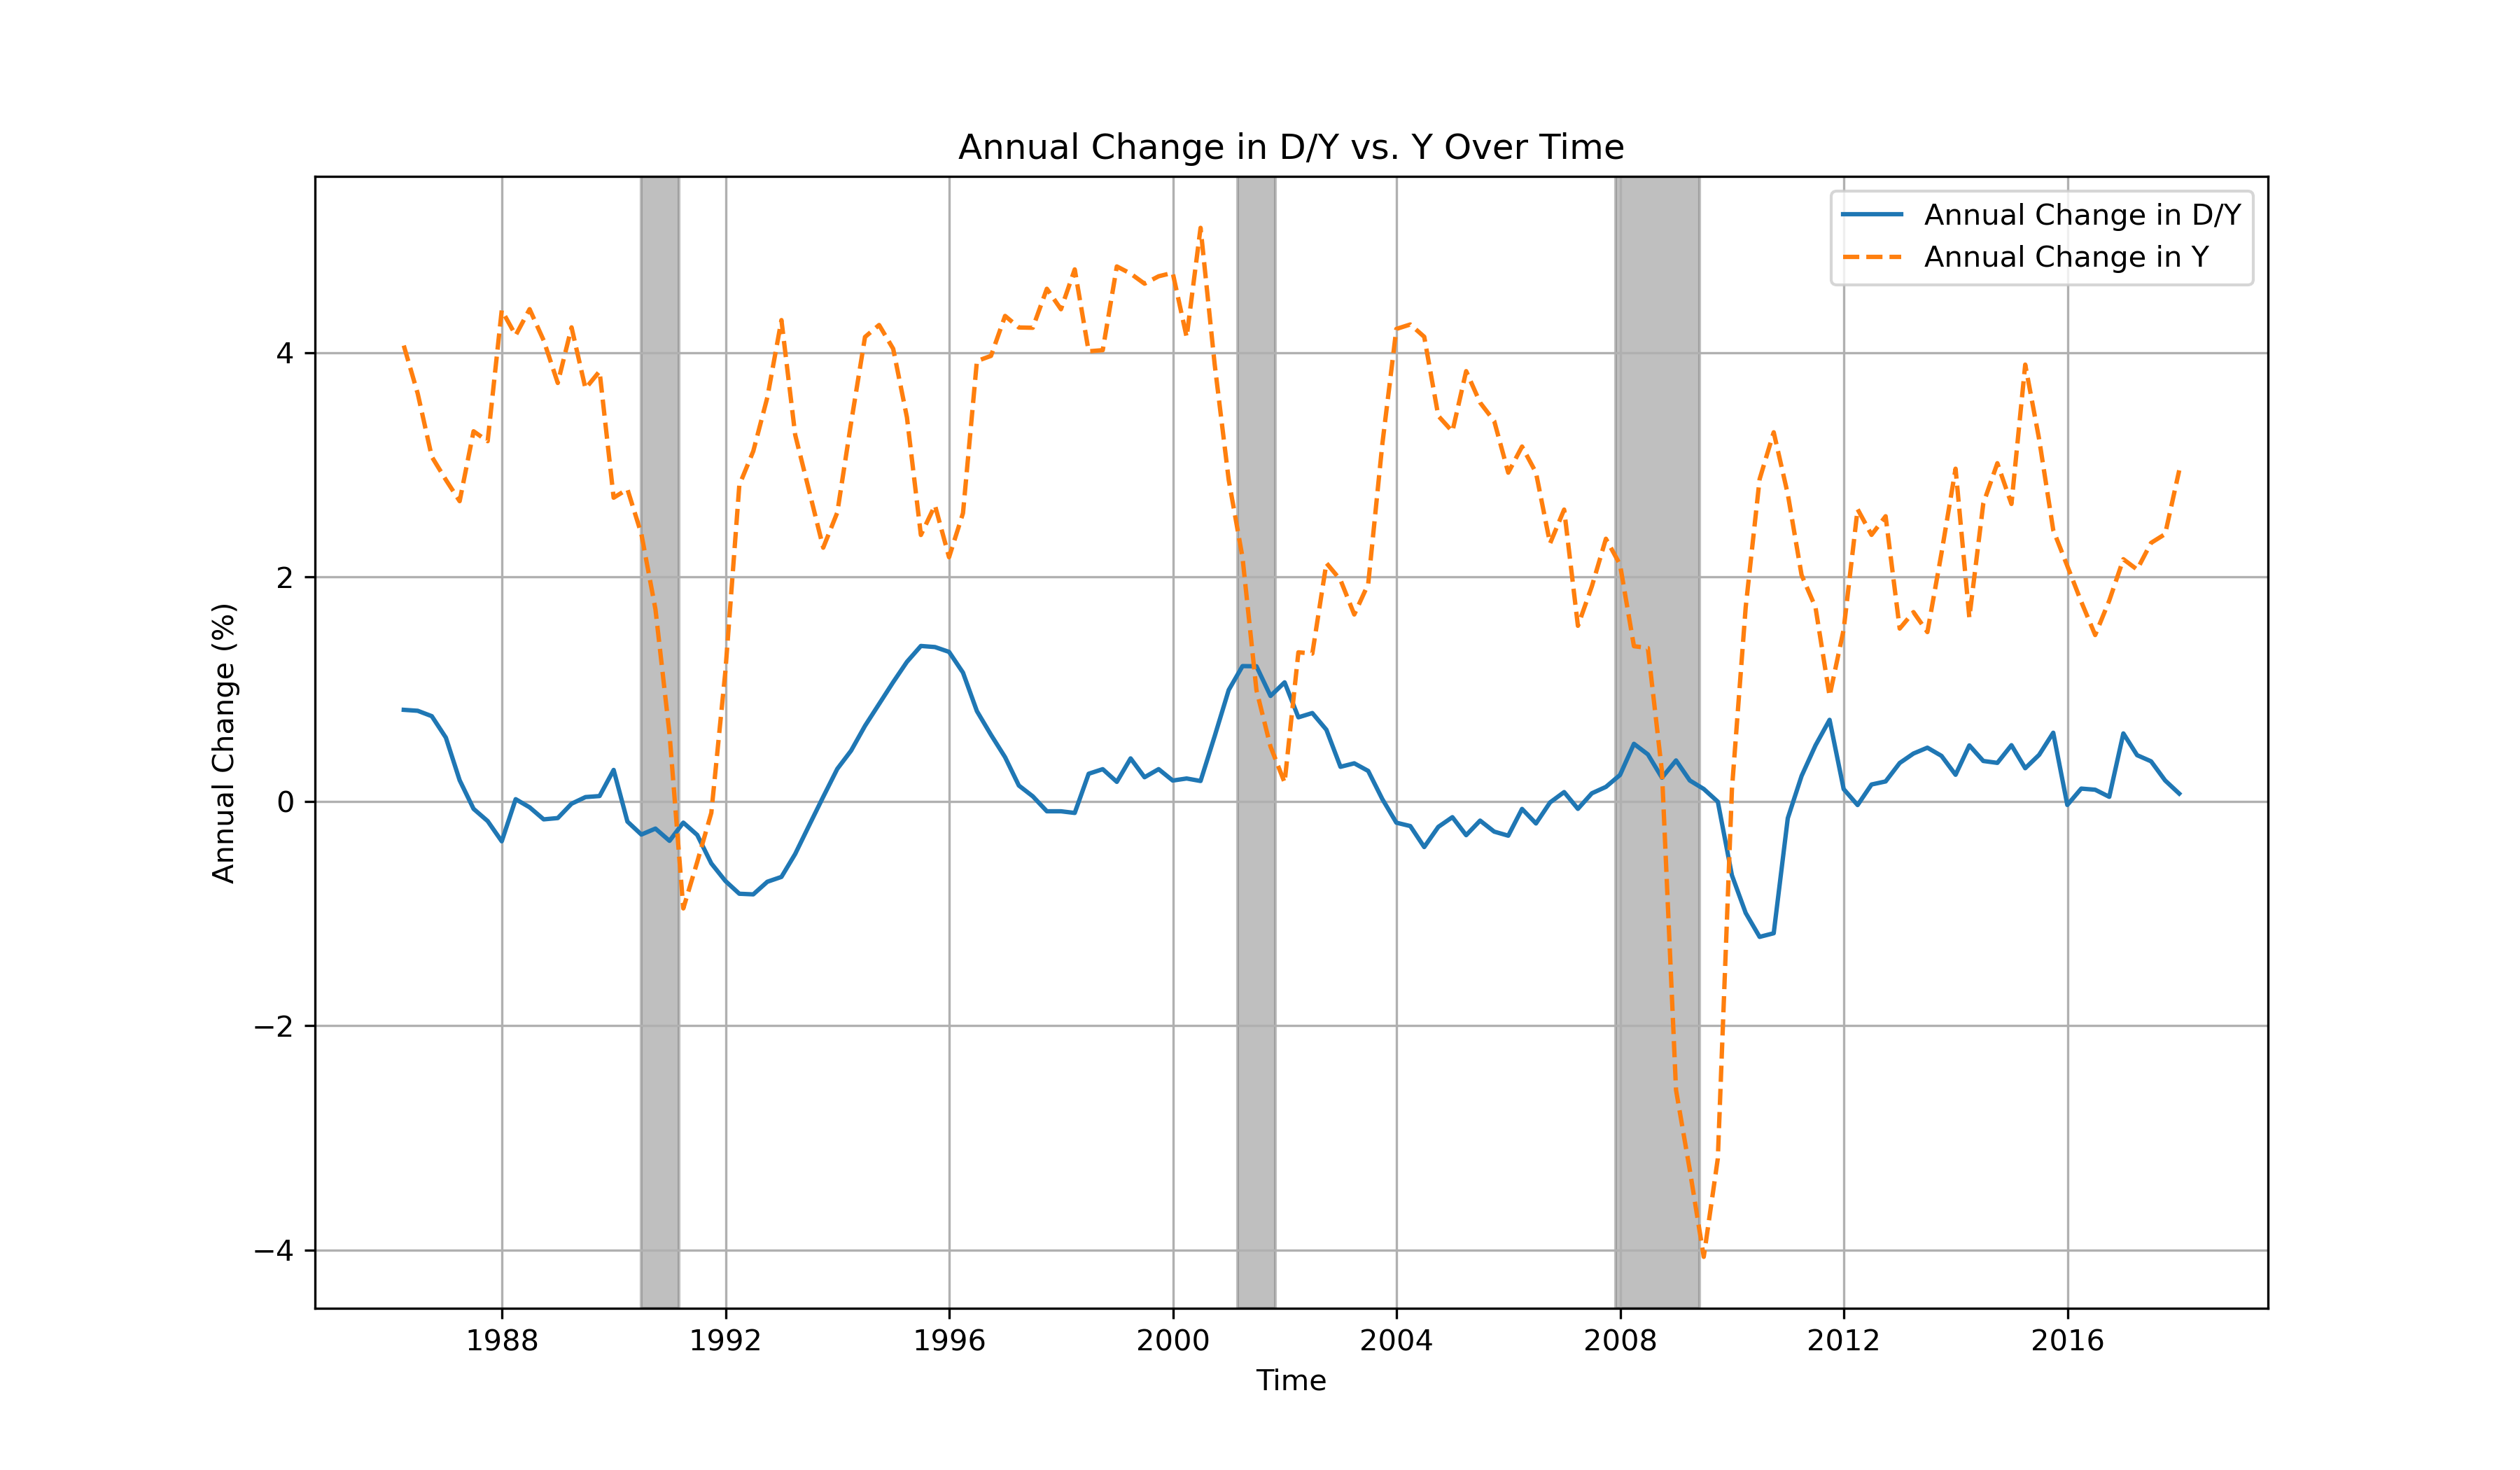
\includegraphics[width=\linewidth]{D_Y_annual_change_vs_Y.png}
\end{subfigure}

\vspace{1em} % Space between the rows

% Second row of two images
\begin{subfigure}{0.45\textwidth}
  \centering
  \includegraphics[width=\linewidth]{CPI_annual_change_vs_Y.png}
\end{subfigure}%
\hspace{0.05\textwidth} % Space between the images
\begin{subfigure}{0.45\textwidth}
  \centering
  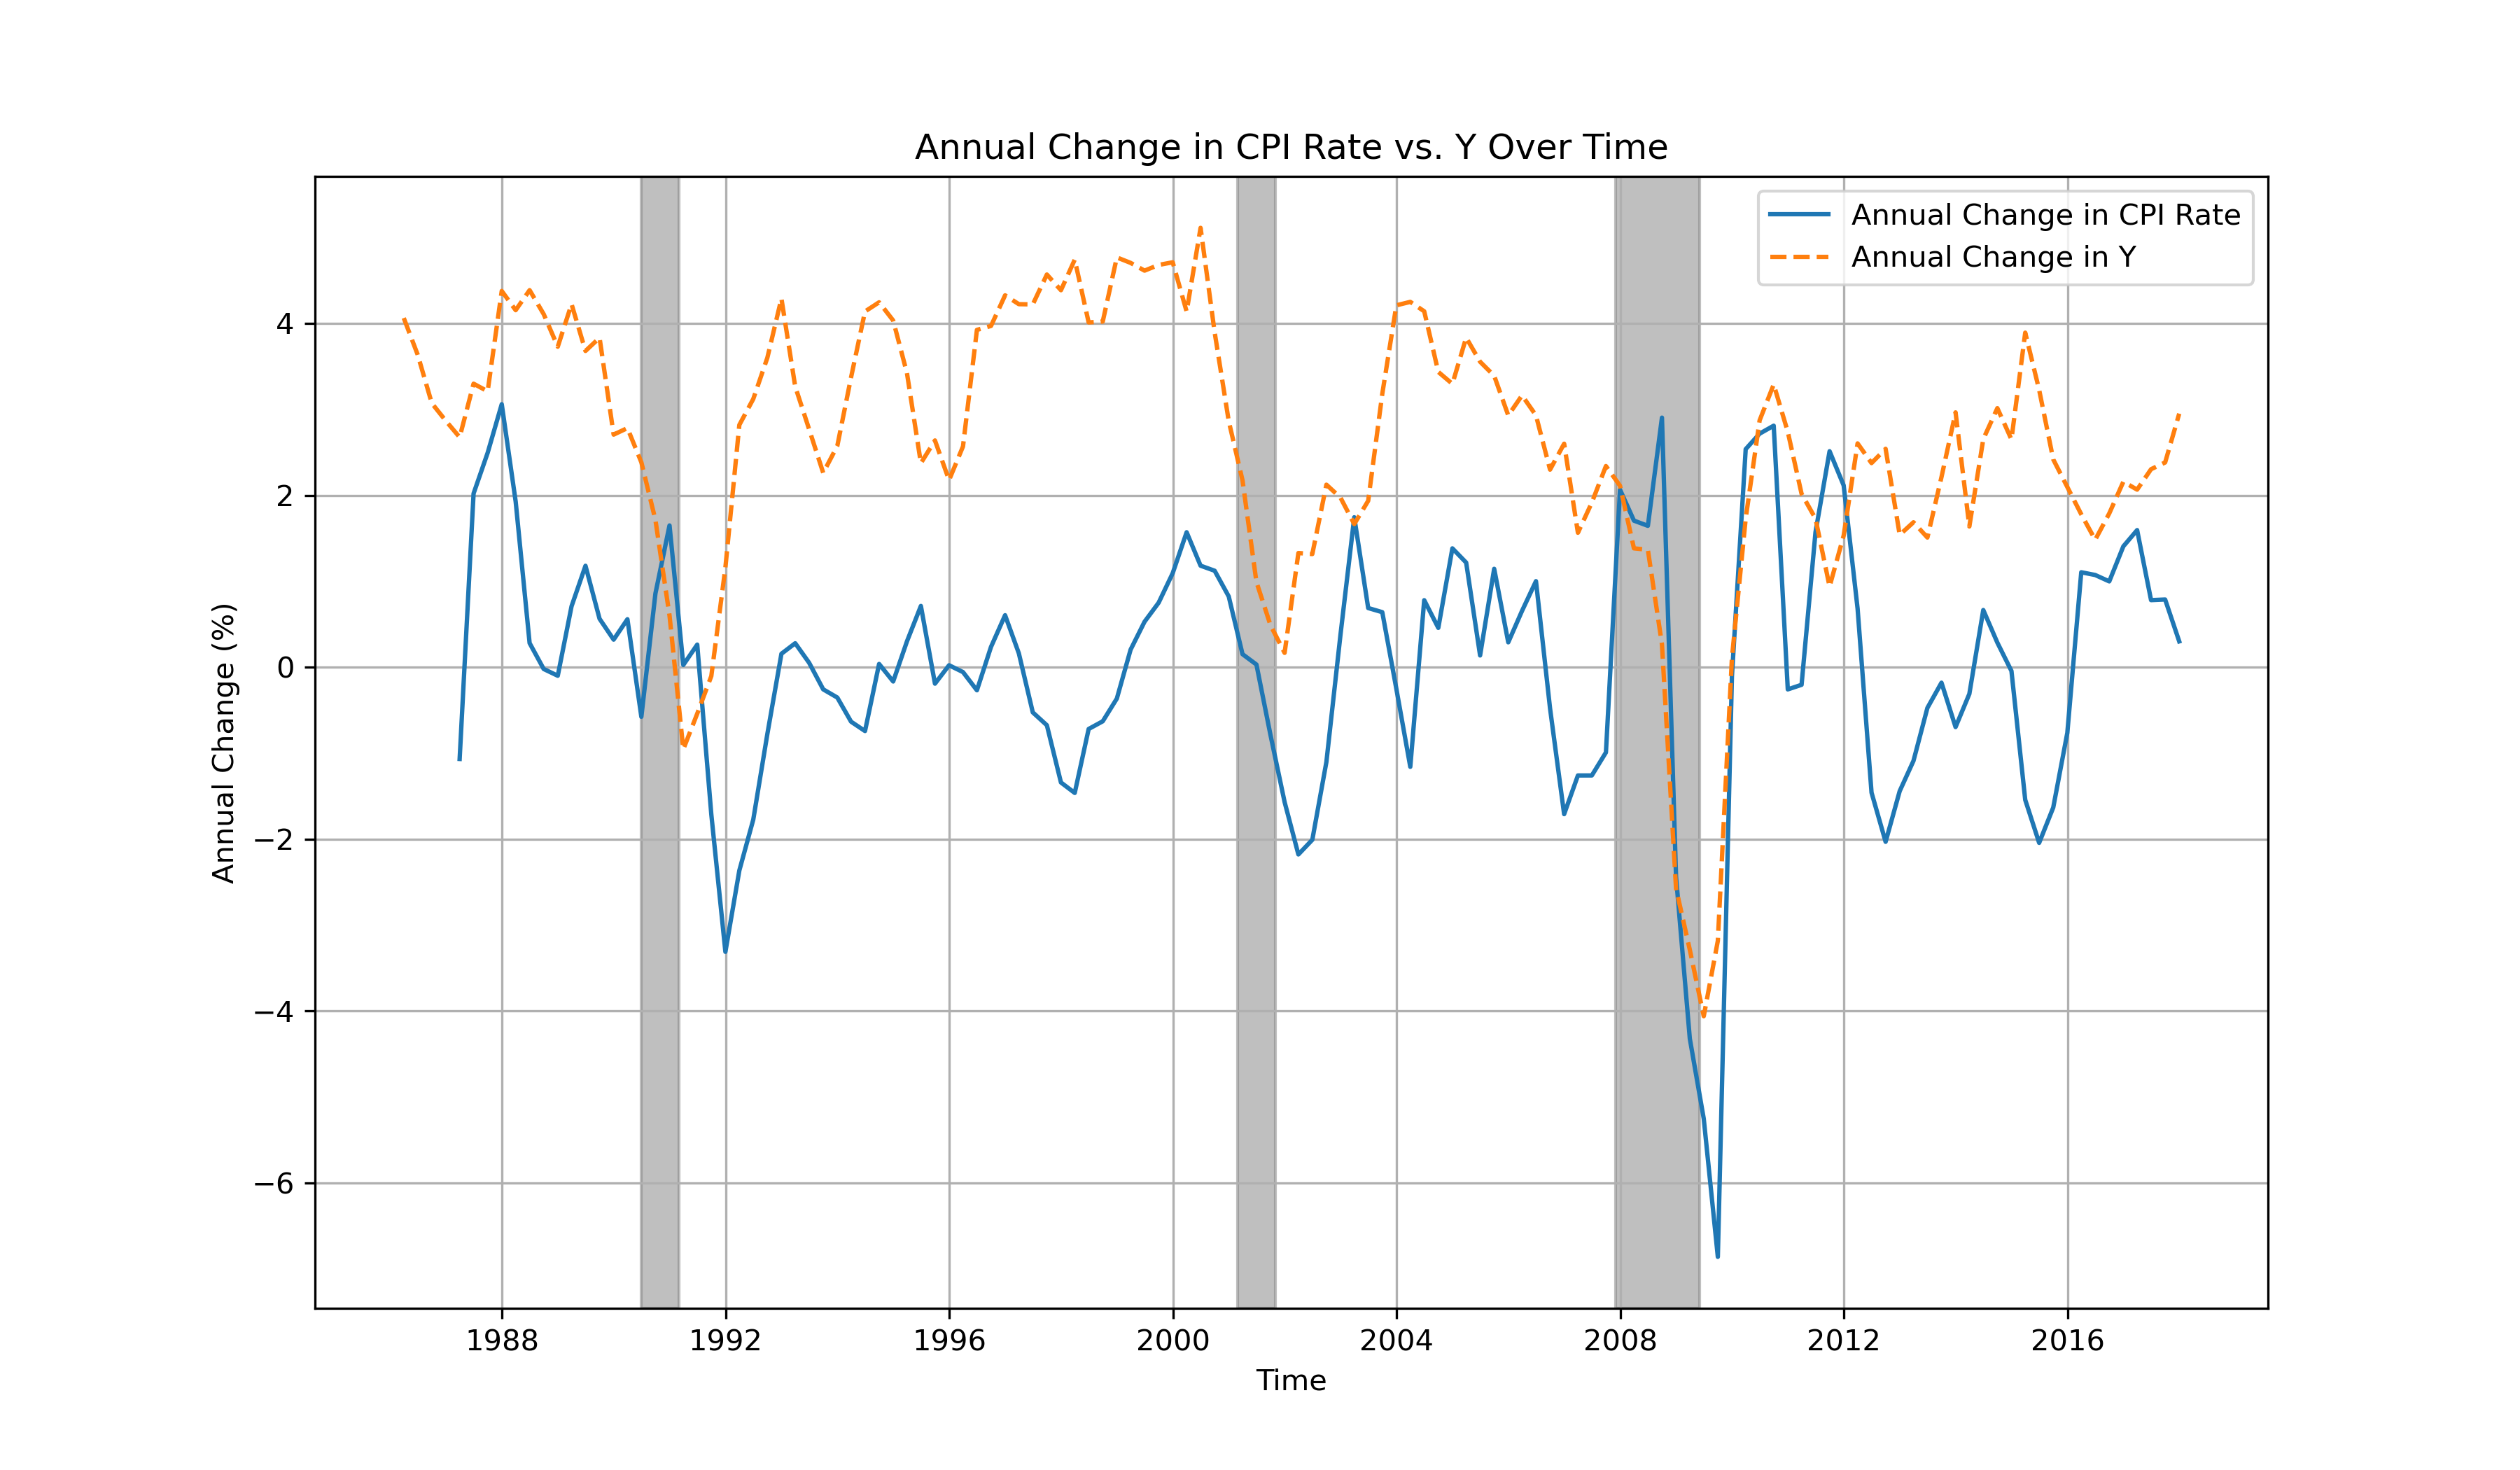
\includegraphics[width=\linewidth]{CPI Rate_annual_change_vs_Y.png}
\end{subfigure}

\vspace{1em} % Space between the rows

% Third row of two images
\begin{subfigure}{0.45\textwidth}
  \centering
  \includegraphics[width=\linewidth]{BK_annual_change_vs_Y.png}
\end{subfigure}%
\hspace{0.05\textwidth} % Space between the images
\begin{subfigure}{0.45\textwidth}
  \centering
  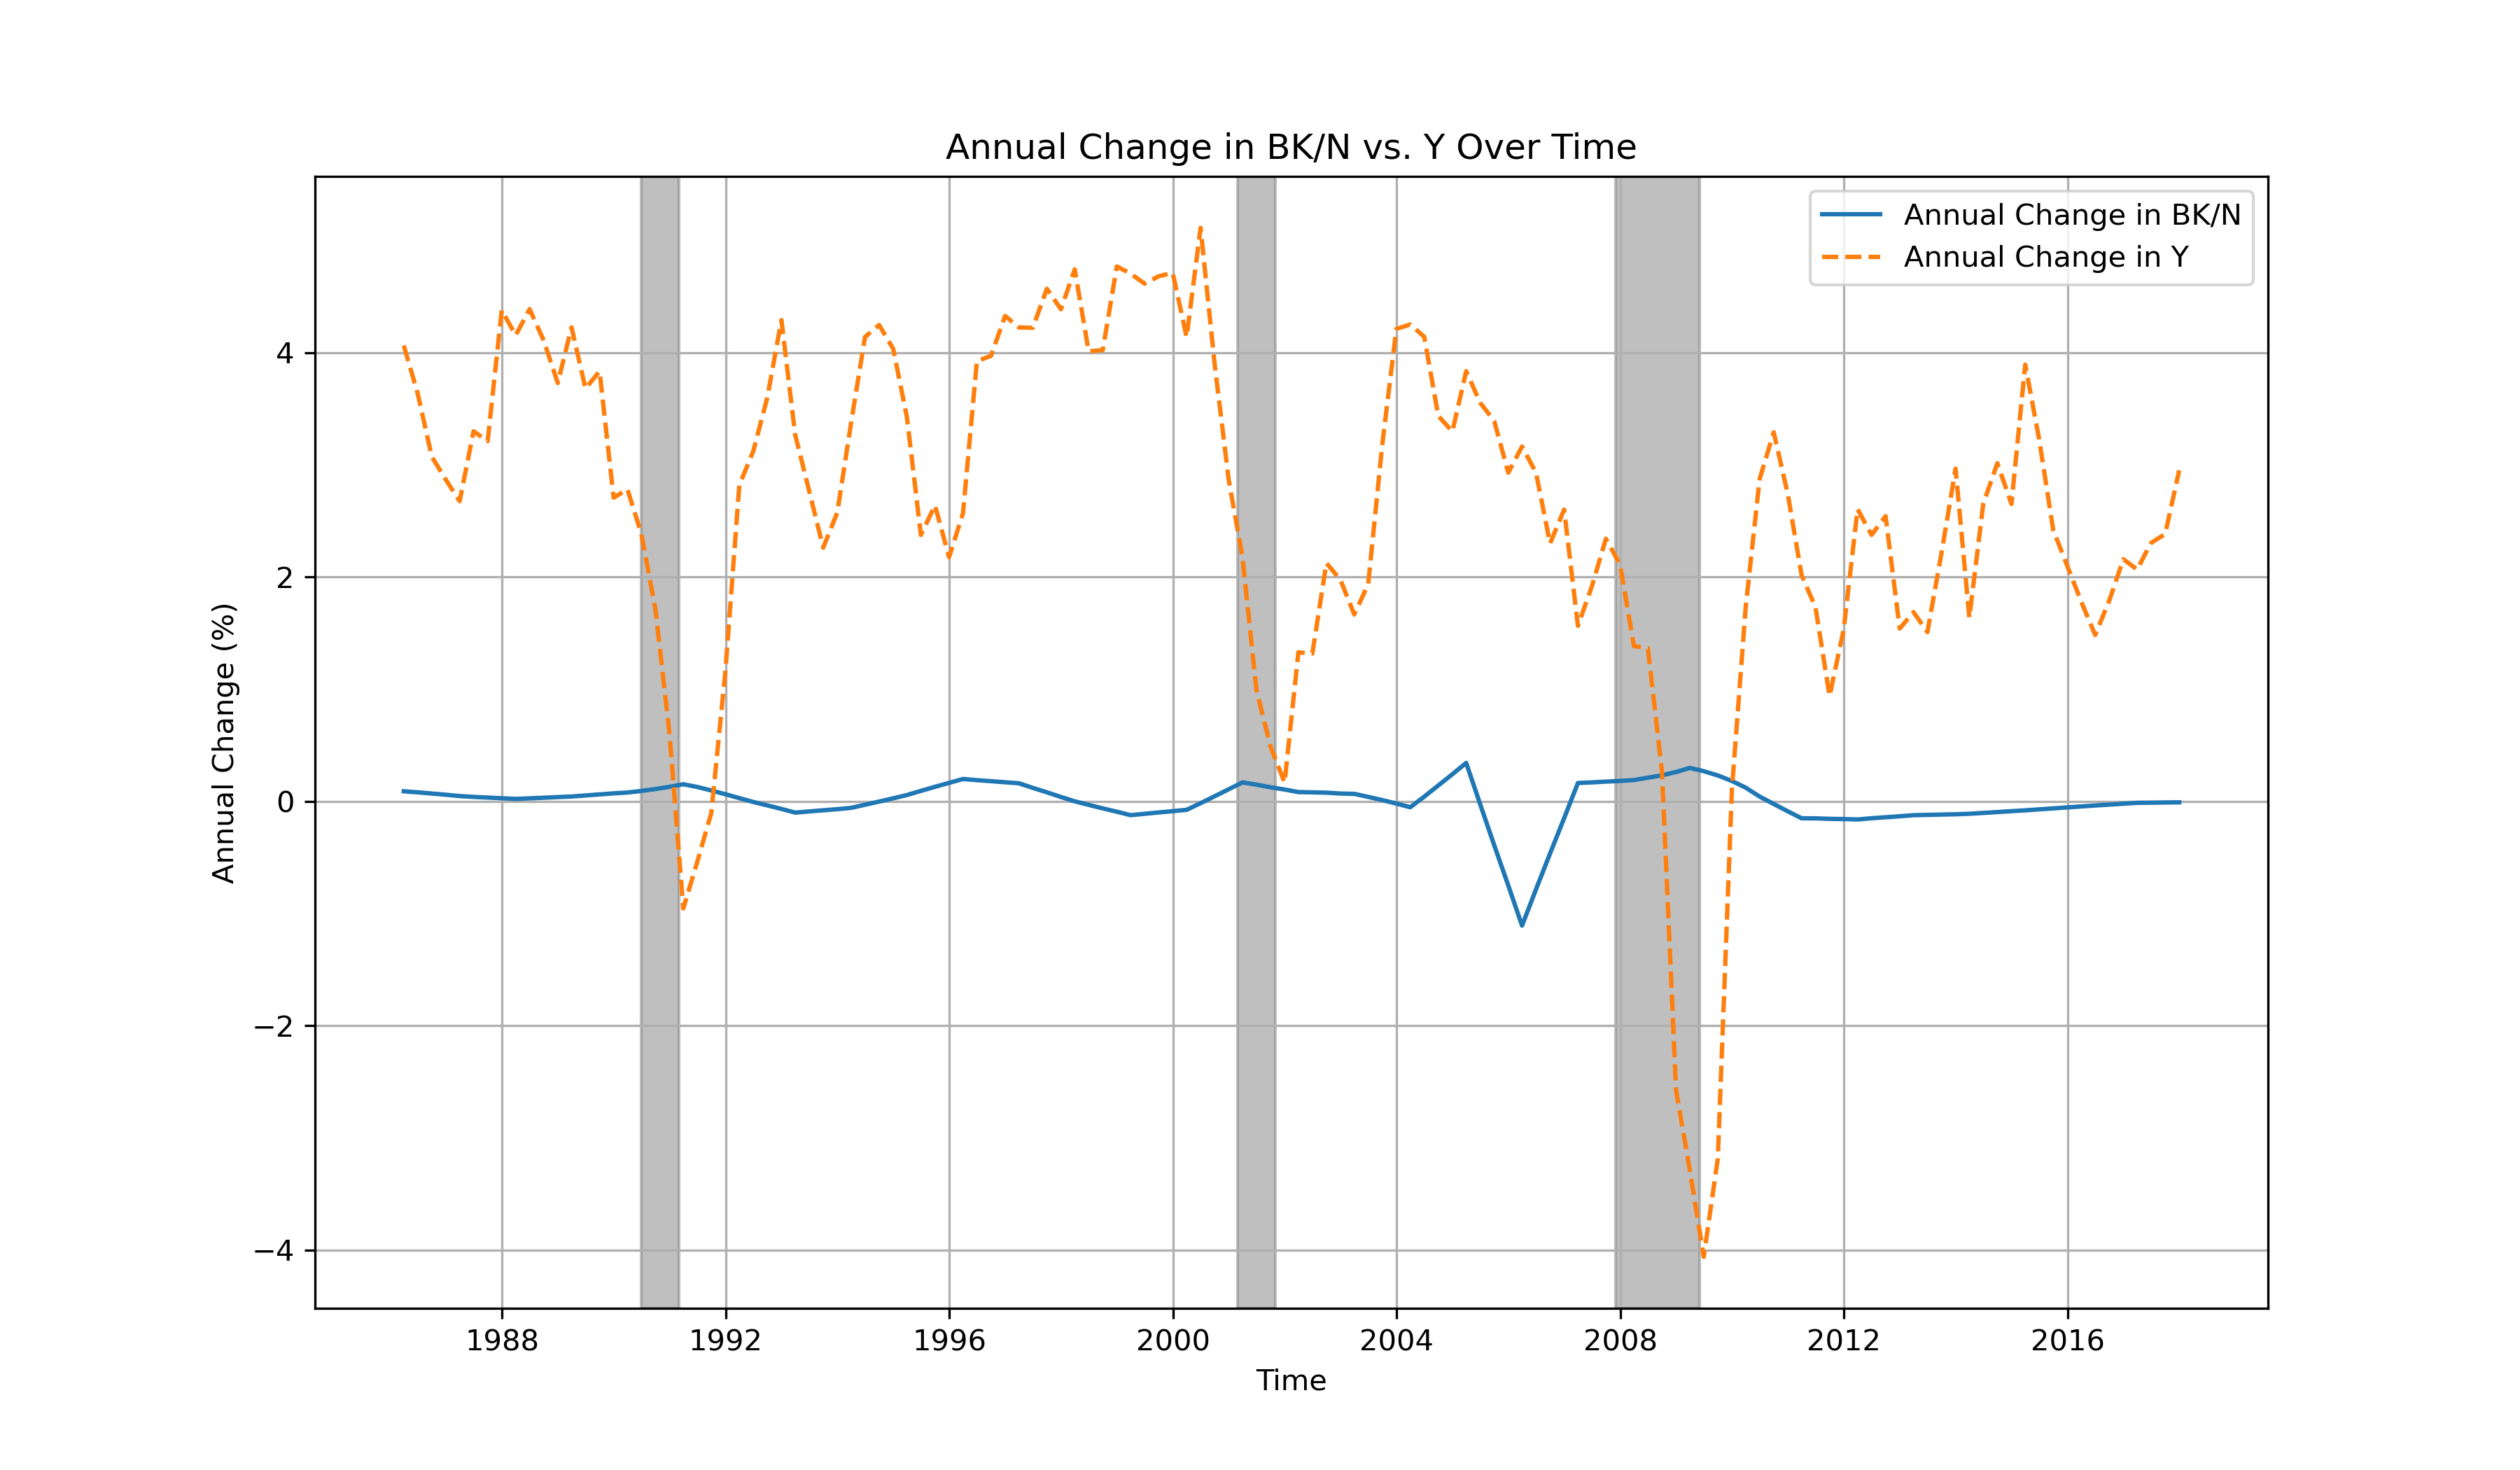
\includegraphics[width=\linewidth]{BK_N_annual_change_vs_Y.png}
\end{subfigure}
\end{figure}


\end{document}

